
\section{用可复核方法提高计算和结论的科学性}

本轮将方法选择落实为四类具体计算：按工程范围和价格阶段建立历史成本参考组；按服务时段核算实际可提供的容量；计算改变收支结论的阈值及参数组合；对真实问卷先审计量表和抽样单位，再给出描述统计。案例沉淀同时解决重复证据的计数问题。每项方法分别说明需要什么数据、程序怎样处理以及会改变哪项判断。

\subsection{原始数据先保留，再核对对象、阶段和分母}

用户提供的AI采集工作簿包含3张表，主表有7条丽水工程、19个字段和14个计算公式。原表逐字节保留；程序分别读取原始数值、公式与缓存结果，14个公式的独立重算均与缓存一致。随后再核实公告来源、金额阶段和面积含义，算术检查与事实核验分别记录。

例如，腾龙一期的正式中标金额为17333131元，92815平方米来自同一完整标段的招标规模；二者可以沿标段编号回查。最高投标限价18997007元及该面积还由公开招标正文同一原件支持。叶坦区块的7732717元在招标正文第9页明确勾选为最高投标限价，第3页给出53021平方米的改造范围。正文中的道路作业面积、总改造范围面积和总建筑面积分别登记。

东升南区有道路面积，却包含多种工程费用；金山新村只记载“总改造面积”，具体面积口径仍需补核；正达阳光城的多名候选人报出同一金额，程序保存一个候选报价记录。由此避免三种错误：把综合费用除成道路单价、把不同面积混作同一分母、把多个投标人当成多个独立改造工程。

\subsection{先形成同口径参考组，再计算金额强度}

GAO成本估算指南要求明确费用范围、单位、价格时期及归一化依据。\cite{gao2020} 本系统按省市、工程类型、工程范围、价格阶段、面积口径和价格年份分组；没有可靠价格指数时保留分年结果。候选报价独立于正式中标，EPC合同独立于施工合同，通信分项独立于整体修缮。

本轮归档27份官方原件，形成20条价格阶段记录；其中24份原件被金额、范围或规模字段直接引用。新增广州3个独立施工合同和上海4个施工中标项目。广州案例的合同金额及总建筑面积来自同一公告；上海案例以明确项目编号和C01施工标段联结中标与招标原件。只有C01或只有相似名称时，不进行跨项目联结。

对已通过口径核验的记录，定义综合金额强度
\begin{equation}
 I_j=\frac{\text{该工程或标段金额（元）}}{\text{明确口径的对应面积（平方米）}}.
\end{equation}
该指标首先服务于同类项目的初步比价；具体施工深度和工程量清单仍在组内逐项比较。受益住宅总建筑面积对应的金额强度，与实际施工的屋面、道路或管线单价分别处理。

\begin{center}\small
\begin{tabular}{@{}L{37mm}rrrrr@{}}
\toprule 参考组 & 项目数 & 记录数 & 最小 & 中位 & 最大\\\midrule

广州2024施工合同 & 2 & 2 & 308.85 & 313.31 & 317.78\\
广州2025施工合同 & 1 & 1 & 289.41 & 289.41 & 289.41\\
上海2026施工中标 & 2 & 2 & 422.65 & 433.23 & 443.81\\

\bottomrule\end{tabular}\end{center}
表中金额强度单位为元/平方米总建筑面积；一个项目的多个公告不增加独立项目数。广州2025年组目前只有一个项目，作为单条参照展示。上述分组不给出总体置信区间，也不把不同城市、年份及价格阶段合成一个杭州报价。广州2024年合同与上海2026年中标之间的差异，需要先核费用内容和价格时期，再安排更细的工程量比较。\cite{gzyouth,gzhong,shcang,shsea}

\subsection{用分时容量纠正月度合计的乐观假设}

服务需求具有时段差异，月平均量会掩盖高峰时段的供给不足。\cite{green2007} 在预约无法改期、服务不能跨时段结转的假设下，设第$t$时段需求为$D_t$、有效容量为$K_t$，则
\begin{equation}
 V=\sum_t\min(D_t,K_t),\qquad
 U=\frac{V}{\sum_tK_t},\qquad
 L=\sum_t\max(0,D_t-K_t).
\end{equation}
这里$V$为服务人次，$U$为容量利用率，$L$为未满足需求人次。由于
\begin{equation}
 \sum_t\min(D_t,K_t)\leq\min\!\left(\sum_tD_t,\sum_tK_t\right),
\end{equation}
月合计计算应被理解为需求可在容量间匹配时的上限。演示中两时段需求为80、20人次，容量各为50人次；分时结果为70人次、未满足30人次、利用率70\%，月合计上限则为100人次。系统同时显示两种结果及30人次的高估量。

界面已支持逐时段输入需求、场次、每场容量及其依据；启用后按分时记录计算。一个时段类别内部仍需说明需求能够匹配该类场次。当前保留独立资源检查，共用场地需要先明确分配；研究并未引入未经校准的随机排队或预约改期模型。

\subsection{用收支切换值说明结论离边界有多远}

Green Book将敏感性分析与切换值用于识别改变方案判断的关键条件。\cite{greenbook2026} 月度运营核算先区分运营方现金与财政支付。设服务人次为$V$、收费比例为$q$、每收费人次价格为$p$、每人次变动成本为$v$、固定运营支出为$F$，其他经营收入为$R_o$、政府购买服务为$G_p$、运营补贴为$S$、其他支持为$H$，则
\begin{equation}
 \Pi=V(qp-v)+R_o+G_p+S+H-F.
\end{equation}
政府直接支付的其他运营费用另列，不重复进入运营方支出；财政支出按政府购买服务、补贴和政府直接支付汇总。建设投资、贷款本息和折旧沿用建设经济模型。

对单一服务，保持价格、收费比例、单位变动成本及其他收支不变，且$qp-v>0$时，保本人次为
\begin{equation}
 V^*=\left\lceil\frac{\max(0,F-R_o-G_p-S-H)}{qp-v}\right\rceil.
\end{equation}
程序同时核对$V^*$是否超过登记容量；在当前服务量保持不变的条件下，另算最低收费和最低收费比例。若收费比例阈值超过1、所需人次超过容量或关键分母为0，直接显示对应条件，而不以总分抵消。

基准演示设月容量520人次、需求400人次、收费比例40\%、每收费人次10元、每服务人次变动成本2元、固定支出10000元、其他经营收入1000元、政府购买服务2000元和补贴6000元。按同一正式计算函数得到：
\begin{center}\small
\begin{tabular}{@{}L{55mm}rL{70mm}@{}}
\toprule 指标 & 结果 & 对判断的具体影响\\\midrule

运营现金结余 & -200元/月 & 基准输入仍有现金缺口\\
按当前服务量所需补贴 & 6200元/月 & 比演示的6000元补贴多200元\\
保本人次 & 500人次/月 & 达到容量的96.15\%，仍需取得相应需求\\
保持400人次时最低收费 & 11.25元/收费人次 & 固定需求的切换值；调价后的需求需另估计\\
保持400人次时最低收费比例 & 45\% & 保持10元收费和其他条件不变\\

\bottomrule\end{tabular}\end{center}
登记容量满负荷时，现金结余只有40元/月；固定支出增至11000元时，保本需要1000人次，超过520人次容量。这比仅展示“积极情景不亏损”更具体地指出了需要核实的固定费用、需求及补贴条件。

\begin{figure}[htbp]
\centering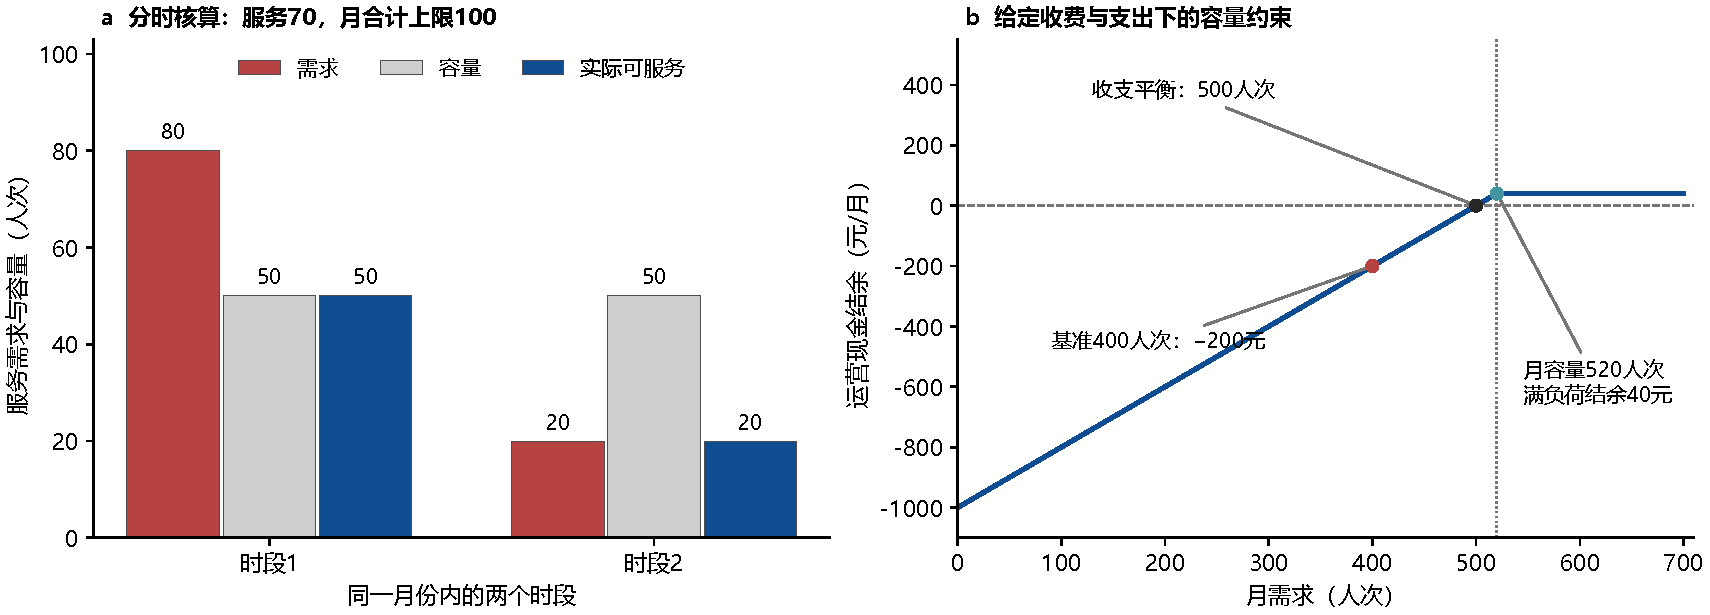
\includegraphics[width=\linewidth]{docs/figures/operations-scientific-checks.pdf}
\caption{同一核算函数的机制检验。a为不可跨时段结转的容量例子；b为给定收费、支出与补贴下的月度需求压力测试。全部为明确标注的演示输入，图中现金边界与表中阈值来自同一结果记录。}
\label{fig:scientific-operations}
\end{figure}

\subsection{把参数范围、单参影响和组合结果一起保存}

系统增加逐参数的下界、基准、上界、范围来源、取得日期及适用说明。单参数分析每次只改一个输入，并调用同一核算函数；组合分析枚举最多6个参数的端点组合。来源不明的百分比不能作为经验分布。\cite{gao2020} 本轮演示以需求倍率0.7至1.3、固定支出9000至11000元测试计算机制，范围性质明确标为人工压力设定。

\begin{center}\small
\begin{tabular}{@{}L{49mm}rrrr@{}}
\toprule 改变的参数 & 下界结余 & 基准结余 & 上界结余 & 结余跨度\\\midrule

固定支出：月度现金事项 & 800 & -200 & -1200 & 2000\\
活动服务：服务需求倍率 & -440 & -200 & 40 & 480\\
\bottomrule\end{tabular}\end{center}
结余及跨度单位均为元/月。四个参数端点组合得到的现金结余为-1440至1040元/月，最大缺口为1440元/月。固定支出的单参跨度为2000元，大于需求变化的480元；在这组演示范围内，固定费用依据更值得优先补充。

这些输出称为“已测试参数组合范围”。若要估计亏损概率或概率覆盖区间，还需有输入分布与依赖关系的依据。JCGM 101要求先依据知识指定输入分布或联合分布，再进行传播计算。\cite{jcgm2008} 本轮不以任意均匀或三角分布把压力测试包装成真实风险概率。

\subsection{真实问卷先审计量表，再按社区重采样}

杭州研究论文提供了居民公共服务评价的公开原始附件。\cite{hangzhou2026} 本轮实读附件为2236份、38个小区、84个字段；论文分析部分报告2202份、36个小区，所检查材料未提供可复现的逐条筛选规则。因此这里明确使用原附件描述口径。程序不保存IP、问卷编号、访员、社区名称或个体记录，只保留计数及统计结果。

量表编码经原附件标签核对为：1非常满意、2基本满意、3一般、4不满意、5非常不满意。本轮将代码1、2合计为满意，中性单列。社区内部观测存在共同环境，方差评估应考虑群集结构。\cite{cdcvariance} 以小区为重采样单位，每次有放回抽取38个小区、保留小区内全部受访者，重算总满意人数除以总有效人数；重复10000次，固定随机种子20261013，取2.5\%和97.5\%分位。

\begin{center}\small
\begin{tabular}{@{}L{48mm}rrr@{}}
\toprule 原附件评价项目 & 满意人数 & 满意比例(\%) & 社区构成敏感区间(\%)\\\midrule

社区服务总体评价 & 910 & 40.70 & 34.65—46.78\\
健身及文化活动场地改造评价 & 934 & 41.77 & 35.27—48.01\\
社区食堂改造评价 & 781 & 34.93 & 29.29—40.74\\
社区养老设施改造评价 & 844 & 37.75 & 31.64—44.11\\
社区幼育设施改造评价 & 801 & 35.82 & 30.68—40.99\\
\bottomrule\end{tabular}\end{center}
若将同一批受访者视为独立样本，总体服务满意比例的Wilson区间仅为38.68\%至42.75\%，明显更窄。\cite{nistwilson} 社区整组结果展示样本社区构成变化的影响；缺少总体抽样权重时，保留为原附件的描述与敏感性结果。满意度、实际到访率和付费采用率分别采集，不能互相代入。

\subsection{用冻结预测和独立对象核验，而非用演示自证准确}

当前应用可冻结预测输入、计算版本、证据和时间，再登记同一中心完整月份的原始台账，保存实际减预测的误差和绝对误差。实际值为0时不计算百分比误差。目标月开始前冻结才归入前瞻对照；事后重建只作历史回放。

后续跨社区检验按社区分组，同一社区的居民记录不能随机拆入训练与测试两侧；跨期检验以较早月份校准、较晚月份验证。数据清理、参数确定和阈值选择只使用校准部分。\cite{groupcv} 本轮已将真实问卷审计、确定性机制检验和月度实绩接口分别实现，实际运营台账尚待取得。

措施展示也采用明确计数单位：项目、案例/规则性质及措施类别相同的记录形成一个默认折叠的措施组，展开后保留不同楼栋、阶段、来源和原卡。宽泛类别中不同原文名称仍可逐项查看。重复提取同一项目、同一来源版本、完全相同字段的记录时复用原卡，不重置复核状态；不同金额、对象或阶段继续分别保存。由此避免把多个原文片段或重复提取误当作多个独立案例。

\subsection{程序应用与复现入口}

现有项目工作台已接入分时录入、收支切换值、带范围依据的敏感性和组合结果；历史工程库支持按面积口径及价格年筛选、显示同口径参考组和排除原因。报告导出保留来源、固定条件、缺项及计算结果，原冻结版本按原值回读。

技术核验分三层：公式与边界测试检查容量守恒、分母和费用重复；HTTP与界面检查录入、保存、读回与导出；真实决策效果留待实际运营台账和独立项目评测。复现采用同一计算入口，表格和图形读取生成结果，关键源文件如下：
\begin{itemize}
\item 月度计算与科学核验：\path{services/capabilities/community_operations.py}、\path{services/capabilities/operations_science.py}。
\item 演示结果复现：\path{scripts/build-scientific-methods-evidence.py}；造价分组复现：\path{scripts/verify-expanded-cost-library.ts}。
\item 用户表接收：\path{scripts/intake-historical-projects-workbook.py}；公开问卷审计：\path{scripts/audit-hangzhou-survey.py}。
\end{itemize}
